\documentclass[tikz]{standalone}
\usetikzlibrary{shapes,arrows.meta}
\begin{document}
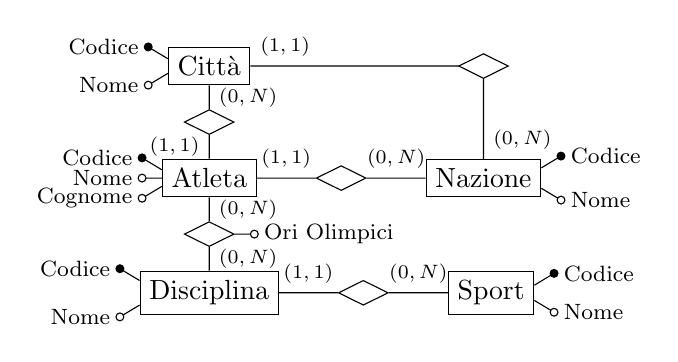
\begin{tikzpicture}
    \draw

    %%* Attributi:
    %%  node[draw, circle, inner sep=1pt, fill=black]{}node[right]{\footnotesize A}
    %%? Distanza orizzontale: E -(0.25,0.x)- A
    %%? Distanza verticale: E -(0,x * 0.22)- A

    %%* Cardinalità:
    %%  node[below right]{\scriptsize $(0,N)$}
    %%  node[above right]{\scriptsize $(0,N)$}
    %%  node[midway, above]{\scriptsize $(0,N)$}

    %%* Relazione:
    %%  node[draw, diamond, shape aspect=2, inner sep=3pt, anchor=90](r1){}
    %%  node[draw, diamond, shape aspect=2, inner sep=0.2pt, anchor=180](r2){R2}

    %%* Entità:
    %%  node[draw, rectangle, anchor=90](e1){}
    %%? Distanza verticale: E -(0.3)- R -(0.3) E
    %%? Distanza orizzontale: E -(0.75)- R -(0.75)- E

    %%* Città
    (0,0)node[draw, rectangle, anchor=180](e1){Città}
    (e1.270)--++(0,-0.3)node[draw, diamond, shape aspect=2, inner sep=3pt, anchor=90](r1){}node[midway, right]{\scriptsize $(0,N)$}

    
    (e1.190)--++(-0.25,-0.15)node[draw, circle, inner sep=1pt, fill=white]{}node[left]{\footnotesize Nome}
    (e1.170)--++(-0.25,0.15) node[draw, circle, inner sep=1pt, fill=black]{}node[left]{\footnotesize Codice}


    %%* Atleta
    (r1.270)--++(0,-0.3)node[draw, rectangle, anchor=90](e2){Atleta}node[midway, left]{\scriptsize $(1,1)$}
    (e2.0)--++(0.75,0)node[draw, diamond, shape aspect=2, inner sep=3pt, anchor=180](r2){}node[midway, above]{\scriptsize $(1,1)$}
    (e2.270)--++(0,-0.3)node[draw, diamond, shape aspect=2, inner sep=3pt, anchor=90](r3){}node[midway, right]{\scriptsize $(0,N)$}

    
    (e2.190)--++(-0.25,-0.15)node[draw, circle, inner sep=1pt, fill=white]{}node[left]{\footnotesize Cognome}
    (e2.180)--++(-0.25,0)node[draw, circle, inner sep=1pt, fill=white]{}node[left]{\footnotesize Nome}
    (e2.170)--++(-0.25,0.15) node[draw, circle, inner sep=1pt, fill=black]{}node[left]{\footnotesize Codice}



    %%* Nazione
    (r2.0)--++(0.75,0)node[draw, rectangle, anchor=180](e3){Nazione}node[midway, above]{\scriptsize $(0,N)$}
    (e3.90)node[above right]{\scriptsize $(0,N)$}|-(e1.0)node[above right]{\scriptsize $(1,1)$}node[midway, draw, diamond, shape aspect=2, inner sep=3pt, fill=white](r4){}

    (e3.350)--++(0.25,-0.15)node[draw, circle, inner sep=1pt, fill=white]{}node[right]{\footnotesize Nome}
    (e3.10)--++(0.25,0.15) node[draw, circle, inner sep=1pt, fill=black]{}node[right]{\footnotesize Codice}


    %%* Disciplina
    (r3.270)--++(0,-0.3)node[draw, rectangle, anchor=90](e4){Disciplina}node[midway, right]{\scriptsize $(0,N)$}
    (r3.0)--++(0.25,0)node[draw, circle, inner sep=1pt, fill=white]{}node[right]{\footnotesize Ori Olimpici}
    (e4.0)--++(0.75,0)node[draw, diamond, shape aspect=2, inner sep=3pt, anchor=180](r5){}node[midway, above]{\scriptsize $(1,1)$}

    (e4.190)--++(-0.25,-0.15)node[draw, circle, inner sep=1pt, fill=white]{}node[left]{\footnotesize Nome}
    (e4.170)--++(-0.25,0.15) node[draw, circle, inner sep=1pt, fill=black]{}node[left]{\footnotesize Codice}

    %%* Sport
    (r5.0)--++(0.75,0)node[draw, rectangle, anchor=180](e5){Sport}node[midway, above]{\scriptsize $(0,N)$}

    
    (e5.350)--++(0.25,-0.15)node[draw, circle, inner sep=1pt, fill=white]{}node[right]{\footnotesize Nome}
    (e5.10)--++(0.25,0.15) node[draw, circle, inner sep=1pt, fill=black]{}node[right]{\footnotesize Codice}


    ;
\end{tikzpicture}
\end{document}